\documentclass{article}
\usepackage{listings}
\usepackage{xcolor}
\usepackage{graphicx}

\title{MPI File Transfer System Design and Implementation}
\author{
    Vu Hai Thien Long (22BI13268) \\
    Luu Linh Ly (22BI13269) \\
    Nguyen Duc Duy (22BI13120) \\
    Le Viet Hoang Lam (22BI13235) \\
    Nguyen Ngoc Nhi (22BI13351)
}
\date{11 December 2024}

\lstdefinestyle{mypython}{
    language=Python,
    backgroundcolor=\color{white},
    basicstyle=\ttfamily\footnotesize,
    keywordstyle=\color{blue},
    commentstyle=\color{gray},
    stringstyle=\color{red},
    numberstyle=\tiny\color{gray},
    numbers=left,
    stepnumber=1,
    numbersep=10pt,
    frame=single,
    rulecolor=\color{black},
    breaklines=true,
    breakatwhitespace=true,
    showstringspaces=false,
    captionpos=b,
}

\begin{document}

\maketitle

\section{Introduction}

This report details the design and implementation of an MPI-based file transfer system. Building upon a TCP-based system, the MPI version leverages parallel processing to enhance performance and scalability.

\section{Choice of MPI Implementation}

We chose \textbf{mpi4py} as our MPI implementation for the following reasons:
\begin{itemize}
    \item \textbf{Seamless Integration with Python}: Allows us to utilize existing Python code with minimal modifications.
    \item \textbf{Comprehensive Documentation}: Facilitates easier development and troubleshooting.
    \item \textbf{Active Community Support}: Ensure access to a wealth of resources and assistance.
    \item \textbf{Performance Efficiency}: Provides robust performance suitable for high-throughput file transfers.
\end{itemize}

\section{Design of the MPI Service}

\subsection{System Architecture}

\begin{figure}[h!]
    \centering
    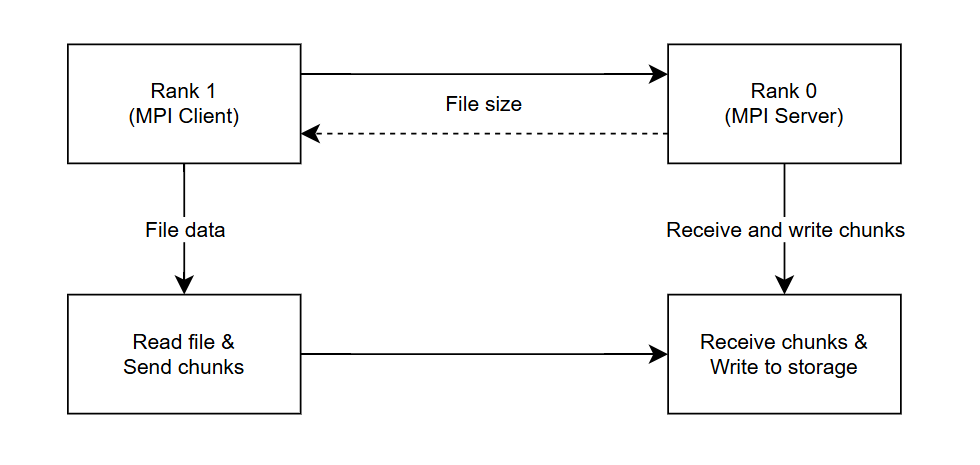
\includegraphics[width=1\textwidth]{mpi_service_design.png}
    \caption{MPI Service Design}
    \label{fig:mpi_service_design}
\end{figure}

The system employs a Master-Worker architecture where the master process coordinates file transfer tasks, and worker processes handle the actual file transmission.

\subsection{Components and Workflow}

\begin{enumerate}
    \item \textbf{Client Process}:
    \begin{itemize}
        \item Initiates a connection to the server.
        \item Sends the file in chunks using MPI communication.
    \end{itemize}
    \item \textbf{Server Process}:
    \begin{itemize}
        \item Listens for incoming file transfer requests.
        \item Receives and assembles the file from chunks.
    \end{itemize}
\end{enumerate}

\section{System Organization}

\begin{figure}[h!]
    \centering
    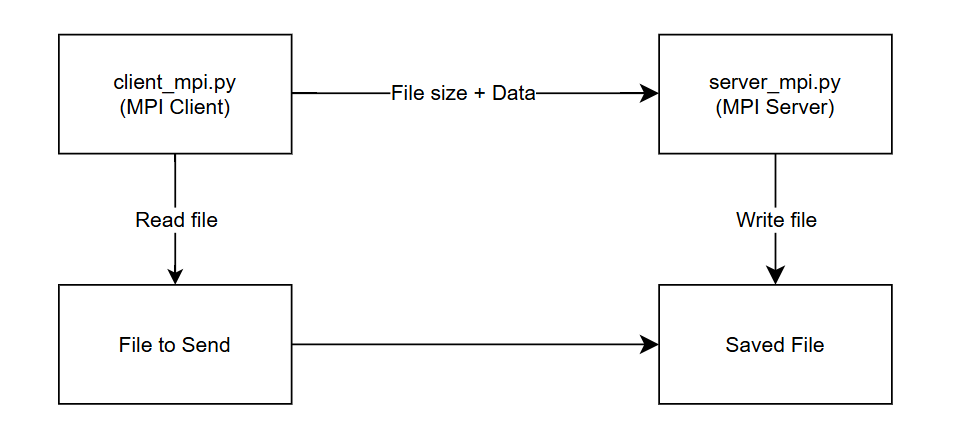
\includegraphics[width=1\textwidth]{mpi_system_organization.png}
    \caption{System Organization Diagram}
    \label{fig:system_organization}
\end{figure}

The system is organized into distinct modules:

\begin{itemize}
    \item \textbf{Client Module}: Handles file reading and sending operations.
    \item \textbf{Server Module}: Manages file reception and storage.
    \item \textbf{Communication Module}: Facilitates MPI-based data transfer between the client and the server.
\end{itemize}

\section{Implementation of File Transfer}

\subsection{Client Code Snippet}

\begin{lstlisting}[style=mypython, caption=MPI Client Implementation]
from mpi4py import MPI
import sys

def send_file(file_path, server_rank=0):
    comm = MPI.COMM_WORLD
    rank = comm.Get_rank()

    if rank == server_rank:
        print("Master process does not send files.")
        return

    try:
        with open(file_path, "rb") as f:
            data = f.read()
    except FileNotFoundError:
        print(f"File {file_path} not found.")
        sys.exit(1)

    file_size = len(data)
    comm.send(file_size, dest=server_rank, tag=11)
    comm.Send([bytearray(data), MPI.BYTE], dest=server_rank, tag=22)
    print(f"File '{file_path}' sent to server.")

if __name__ == "__main__":
    if len(sys.argv) != 2:
        print("Usage: mpirun -n <number_of_processes> python client_mpi.py <file_path>")
        sys.exit(1)

    file_path = sys.argv[1]
    send_file(file_path)
\end{lstlisting}

\subsection{Server Code Snippet}

\begin{lstlisting}[style=mypython, caption=MPI Server Implementation]
from mpi4py import MPI
import sys

def receive_file(output_path="received_file_mpi.txt", client_rank=1):
    comm = MPI.COMM_WORLD
    rank = comm.Get_rank()

    if rank != client_rank:
        print("Only the designated server process receives files.")
        return

    file_size = comm.recv(source=MPI.ANY_SOURCE, tag=11)
    buffer = bytearray(file_size)
    comm.Recv([buffer, MPI.BYTE], source=MPI.ANY_SOURCE, tag=22)

    with open(output_path, "wb") as f:
        f.write(buffer)
    print(f"File received and saved as '{output_path}'.")

if __name__ == "__main__":
    receive_file()
\end{lstlisting}

\section{Roles and Responsibilities}

\begin{itemize}
    \item \textbf{Vu Hai Thien Long}: Implemented the MPI client and handled file reading operations.
    \item \textbf{Luu Linh Ly}: Developed the MPI server and managed file reception.
    \item \textbf{Nguyen Duc Duy}: Created system diagrams and contributed to the LaTeX report.
    \item \textbf{Le Viet Hoang Lam}: Integrated client and server modules and ensured seamless communication.
    \item \textbf{Nguyen Ngoc Nhi}: Coordinated group activities and managed version control.
\end{itemize}

\section{Conclusion}

The MPI-based file transfer system successfully enhances the original TCP-based system by leveraging parallel processing capabilities. The use of `mpi4py` facilitated efficient implementation and scalability, making the system robust for handling multiple file transfers concurrently.

\end{document}
